\documentclass[french]{article}

\usepackage{mathtools, bm}
\usepackage{amssymb, bm}
\usepackage[utf8]{inputenc}
\usepackage[T1]{fontenc}
\usepackage{babel}
\usepackage{amsmath}
\usepackage{graphicx}
\usepackage{eso-pic}
\usepackage{fullpage}
\usepackage{ulem}
\usepackage{ntheorem}
\usepackage{xcolor}
\usepackage{titlesec}
\usepackage{stmaryrd}
\usepackage{calrsfs}
\usepackage[left=2cm,right=2cm,top=2cm,bottom=2cm]{geometry}
\theorembodyfont{\upshape}
\theoremstyle{break}

\titleformat{\section}
   {}% apparence commune au titre et au numéro
   {}% apparence du numéro
   {1em}% espacement numéro/texte
   {\LARGE}% apparence du titre

\titleformat{\subsection}
   {}% apparence commune au titre et au numéro
   {}% apparence du numéro
   {1em}% espacement numéro/texte
   {\large}% apparence du titre

\definecolor{bleuturquoise}{RGB}{30, 81, 122}

\title{Projet base de données}
\author{Julie SAOULI, Maxime GOURGOULHON, Pierre BOUVIER, Geoffrey TANGUY, Jérôme THÉATE}
\date{ENSIMAG | Enseignant encadrant : M. Christophe BOBINEAU | 2017 - 2018 }
\makeatletter
\begin{document}
\renewcommand*\contentsname{\huge{Table des matières\vspace{1cm}}}
\begin{titlepage}
\begin{center}
\text{  }\\
\text{  }\\
\text{  }\\
\text{  }\\
\textbf{{\fontsize{45}{45}\selectfont Projet Base de Données}}\\
\vspace{0.5cm}
\textbf{\LARGE{COMPTE-RENDU}}
\end{center}
\vspace{10cm}
\begin{center}
\makebox[\textwidth]{}
\end{center}

\vspace{4.0cm}
\begin{center}
Pierre BOUVIER \hspace{1.5cm} Maxime GOURGOULHON  \hspace{1.5cm} Julie SAOULI
\end{center}
\hspace{4.2cm} Geoffrey TANGUY \hspace{3cm} Jérôme THÉATE
\vspace{0.2cm}
\begin{center}
\large{\@date}
\end{center}
\end{titlepage}
\clearpage

\begin{Large}
\tableofcontents
\end{Large}
\clearpage







\noindent\textsc{\textcolor{bleuturquoise}{\section{Introduction}}}

L'agence de voyage \textsc{AWHY}, forte de son succès, entreprend sa transformation numérique. Elle tient à numériser ses outils de gestion tout en conservant une étroite collaboration avec ses partenaires. De ce fait, certaines règles d'implémentation devront être respectées afin d'assurer la compatibilité des bases de données communes entre tous les partenaires.\\

Dans le cadre du développement de la société \textsc{AWHY}, nous avons été mandaté pour réaliser la conception et l'implémentation de leur base de données. Ce rapport vous apportera les outils nécessaires à la compréhension de la conception de cette base de données et vous permettra en outre de prendre connaissance des enjeux et des difficultés qui ont permis de privilégier certains axes de réflexion. Enfin, vous y trouverez certains détails quant à nos choix d'implémentation ayant permis de mettre en valeur et d'exploiter le potentiel des bases de données de la société.

\vspace{0.3cm}
\noindent\textsc{\textcolor{bleuturquoise}{\section{Analyse du problème}}}

L'application doit proposer deux vues :
\begin{itemize}
\item une vue \textit{client} permettant à l'utilisateur de créer sa simulation et d'obtenir un numéro de dossier, puis de pouvoir consulter le catalogue de l'agence et ajouter à sa simulation des hôtels, des lieux à visiter et des circuits, et enfin confirmer sa simulation. Il pourra alors se présenter à l'agence avec son numéro de dossier et effectuer sa réservation.
\item une vue \textit{agence} permettant de vérifier la simulation d'un client venu à l'agence, de la modifier si nécessaire et de la valider en lui ajoutant un paiement. L'agence sera capable de consulter la liste des simulations, des réservations et des clients. \\
\end{itemize}

Il sera également vital que de multiples utilisateurs puissent se connecter à la base de données via l'application et la modifier simultanément.
De plus, afin d'assurer la compatibilité avec les applications partenaires, les relations décrivant les villes, hôtels, circuits et lieux à visiter ne devront pas être modifiées. \\

L'analyse du problème nous a conduit à l'identification des propriétés élémentaires et à l'élaboration du schéma-entité association correspondant.


\noindent\textsc{\textcolor{bleuturquoise}{\section{Conception de la base de données}}}

\textsc{\subsection{Propriétés élémentaires}}

\{ nomVille, pays, nomLieu, adresseLieu, descriptifLieu, prix, idCircuit, descriptif, villeDépart, paysDepart, villeArrivee, paysArrivee, nbJoursTotal, prixCircuit, dateDepartCircuit, nbPersonnes, ordre, nbJours, nomHotel, adresseHotel, nbChambresTotal, prixChambre, prixPetitDejeuner, idClient, typeClient, anneeEnregistrement, nomClient, prenomClient, adresseClient, emailClient, telClient, numDossier,
numDossierReservation, numDossierSimulation, datePaiement, infoPaiement, nomClientSimu, prenomClientSimu, nbChambres, dateDepartHotel, dateArriveeHotel, dateVisite, nbPersonnesVisite, nbChambresReservees, nbPetitDejReserves, numDossierReservation \}


\vspace{0.3cm}
\textsc{\subsection{Contraintes de valeur}}
\vspace{0.3cm}

\noindent prix $\geq 0$ \\
nbJours $\geq 0$ \\
nbJoursTotal $\geq 0$ \\
prixCircuit $> 0$ \\
$Ext($ordre$) \subseteq \llbracket 0, ..., Max(Ext($ordre$)\rrbracket$ \\
nbChambresTotal $> 0$ \\
prixChambre $> 0$ \\
prixPetitDejeuner $\geq 0$ \\
typeClient $\in$ {individuel, societe, groupe} \\
$Ext($numDossierReservation$)\cup Ext($numDossierSimulation$) = Ext($numDossier$)$ \\
dateDepartHotel $\leqslant$ dateArriveeHotel \\
nbPersonnesVisite $> 0$ \\
nbChambresReservees $> 0$ \\
nbPetitDejReserves $\geq 0$ \\


\textsc{\subsection{Dépendances fonctionnelles}}


\textsc{Issues du schéma relationnel fourni :}

\noindent nomLieu, nomVille, pays $\rightarrow$ adresseLieu, descriptifLieu, prix\\
\noindent idCircuit $\rightarrow$ descriptif, villeDepart, paysDepart, villeArrivee, paysArrivee, nbJoursTotal, prixCircuit\\
idCircuit, dateDepartCircuit $\rightarrow$ nbPersonnes\\
idCircuit, ordre $\rightarrow$ nomLieu, nomVille, pays, nbJours\\
nomHotel, nomville, pays $\rightarrow$ adresseHotel, nbChambresTotal, prixChambre, prixPetitDejeuner\\
villeDepart, paysDepart $\rightarrow$ nomVille, pays\\
villeArrivee, paysArrivee $\rightarrow$ nomVille, pays\\


\textsc{Issues de notre analyse :}

\noindent idClient $\rightarrow$ nomClient, prenomClient, typeClient, adresseClient, emailClient, telClient, annéeEnregistrement\\
numDossier, idCircuit, dateDepartCircuit $\rightarrow$ nbPersonnesCircuit\\
numDossier, nomHotel, nomVille, pays, dateDepartHotel, dateArriveeHotel $\rightarrow$ nbChambresReservees, nbPetitDejReserves\\
numDossier, nomLieu, nomVille, pays, dateVisite $\rightarrow$ nbPersonnesVisite\\
numDossierReservation $\rightarrow$ datePaiement, infoPaiement, idClient\\
numDossierSimulation $\rightarrow$ nomClientSimu, prenomClientSimu


\textsc{\subsection{Contraintes de multiplicité}}

\textsc{Hôtels :}

\noindent numDossier $-|\twoheadrightarrow$ nomHotel, nomVille, pays\\
nomHotel, nomVille, pays $-|\twoheadrightarrow$ numDossier\\
numDossier, dateDepartHotel, dateArriveeHotel $\twoheadrightarrow$ nomHotel, nomVille, pays\\
nomHotel, nomVille, pays, dateDepartHotel, dateArriveeHotel $\twoheadrightarrow$ numDossier\\
nomVille, pays $-|\twoheadrightarrow$ nomHotel, nomVille, pays\\


\textsc{Lieux à visiter :}

\noindent numDossier $-|\twoheadrightarrow$ nomLieu, nomVille, pays\\
nomLieu, nomVille, pays $-|\twoheadrightarrow$ numDossier\\
numDossier, dateVisite $\twoheadrightarrow$ nomLieu, nomVille, pays\\
nomLieu, nomVille, pays, dateVisite $\twoheadrightarrow$ numDossier\\
nomVille, pays $-|\twoheadrightarrow$ nomLieu, nomVille, pays\\



\textsc{Circuits :}

\noindent numDossier $-|\twoheadrightarrow$ idCircuit, dateDepartCircuit\\
idCircuit, dateDepartCircuit $-|\twoheadrightarrow$ numDossier\\
idCircuit $\twoheadrightarrow$ idCircuit, dateDepartCircuit\\
nomLieu, nomVille, pays $-|\twoheadrightarrow$ idCircuit, ordre\\
nomVille, pays $-|\twoheadrightarrow$ villeDepart, paysDepart\\
nomVille, pays $-|\twoheadrightarrow$ villeArrivee, paysArrivee \\

\newpage

\textsc{Clients :}

\noindent idClient $\twoheadrightarrow$ numDossierReservation\\
idClient $-|\twoheadrightarrow$ numDossierSimulation \\


\textsc{\subsection{Autres contraintes}}

\noindent “Un dossier contient au moins une réservation d'hôtel, circuit ou lieu à visiter.”\\
“Les informations de simulation (nomClientSimu, prenomClientSimu) peuvent correspondre à un client (et un seul) ou non.” \\
“Un circuit commence par une étape de départ et se termine par une étape d’arrivée. Tout circuit contient au moins deux étapes : le départ et l’arrivée.”\\
“Au paiement, et pour permettre la réservation du voyage, il faut vérifier la disponibilité des hôtels et circuits réservés, c'est-à-dire que le nombre de chambres/places disponibles est compatible avec le nombre de chambres/places réservées.”

\newpage


\textsc{\textcolor{bleuturquoise}{\section{Schéma Entité-Association}}}

\begin{figure}[!h]
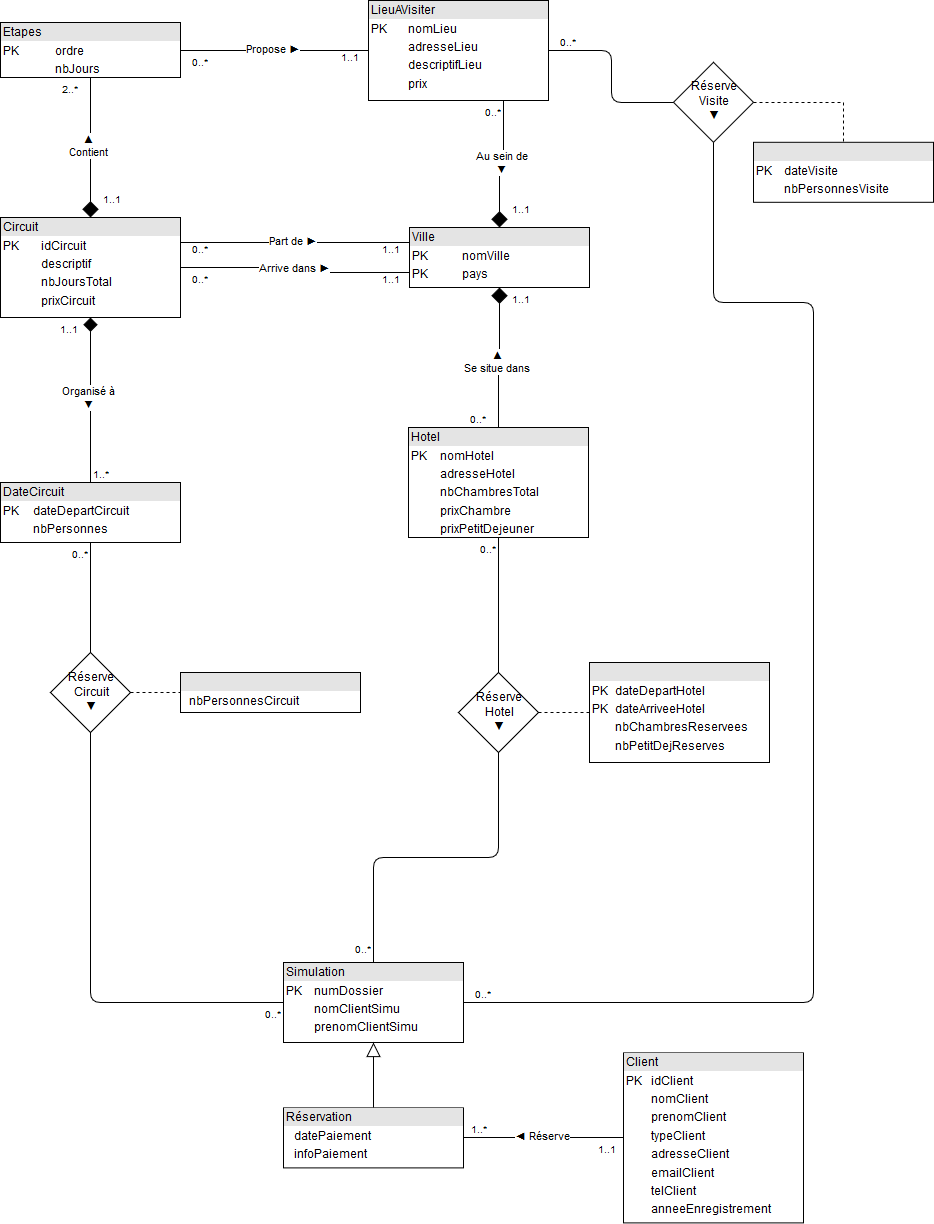
\includegraphics[scale=0.47]{diagrams/schema_uml_rapport.png}
\end{figure}


\newpage
\textsc{\textcolor{bleuturquoise}{\section{Passage au relationnel}}}

\textsc{\subsection{Types d'entités simples}}

\noindent Ville (\underline{nomVille}, \underline{pays}) \\
Circuit (\underline{idCircuit}, descriptif, villeDepart, paysDepart, villeArrivee, paysArrivee, nbJoursTotal, prixCircuit) \\
Client (\underline{idClient}, nomClient, prenomClient, typeClient, adresseClient, emailClient, telClient, anneeEnregistrement) \\
Simulation (\underline{numDossier})


\textsc{\subsection{Types d'entités faibles}}

\textsc{Entités faibles de Ville :}
\vspace{0.3cm}

\noindent Hotel (\underline{nomHotel}, \underline{ville}, \underline{pays}, adresseHotel, nbChambresTotal, prixChambre, prixPetitDejeuner) \\
LieuAvisiter (\underline{nomLieu}, \underline{ville}, \underline{pays}, adresseLieu, descriptifLieu, prix) \\

\textsc{Entités faibles de Circuit :}
\vspace{0.3cm}

\noindent DateCircuit (\underline{idCircuit}, dateDepartCircuit, nbPersonnes) \\
Etapes (\underline{idCircuit}, \underline{ordre}, nomLieu, ville, pays, nbJours)


\textsc{\subsection{Sous-types d'entités}}

\noindent Simulation(\underline{numDossier}, nomClientSimu, prenomClientSimu) \\
\noindent Reservation(\underline{numDossier}, datePaiement, infoPaiement, idClient) \\

Les entités Simulation et Reservation sont des sous-types d'entité de l'entité Dossier(\underline{numDossier}). Nous avons fait le choix de conception qu'un dossier est une simulation ou une réservation et une simulation, c'est-à-dire qu'une simulation payée devient une réservation mais n'est pas supprimé des simulations. Ce choix nous a semblé judicieux afin que l'agence puisse conserver une trace des simulations initiales, même après que celles-ci aient été modifiées par manque de disponibilité. Cela pourrait permettre à l'agence d'adapter son catalogue à la demande.

Par ce choix, renforcé par le faible coût de la clé numDossier et par l'absence d'attributs autres dans Dossier, nous avons décidé de ne pas représenter l'entité Dossier et de dupliquer la clé dans les deux entités Simulation et Reservation.


\textsc{\subsection{Associations}}

Les entités liées à la réservations d'hôtels, de lieux à visiter et de circuits sont issus d'associations entre l'entité Client et les entités Hotel, LieuAvisiter et Circuit. \\

\noindent ReserveHotel (\underline{nomHotel}, \underline{ville}, \underline{pays}, \underline{numDossier}, \underline{dateDepartHotel}, \underline{dateArriveeHotel}, nbChambresReservees, nbPetitDejReserves) \\
ReserveCircuit (\underline{idCircuit}, \underline{dateDepartCircuit}, \underline{numDossier}, nbPersonnesCircuit) \\
ReserveVisite (\underline{nomLieu}, \underline{ville}, \underline{pays}, \underline{numDossier}, \underline{dateVisite}, nbPersonnesVisite)


\textsc{\subsection{Formes normales}}

Toutes les relations sont \textit{3FN} car pour chacune tous les attributs non clés sont pleinement dépendants et directement issus des clés de l'entité à laquelle elles appartiennent. Les relations sont \textit{3FN BCK} car elles sont toutes 3FN et toutes les dépendances fonctionnelles élémentaires se déduisent de la connaissance des clés.

\newpage

\textsc{\textcolor{bleuturquoise}{\section{Analyse des fonctionnalités}}}

Les transactions sont sérialisables afin d'isoler chaque utilisateur et permettre des transactions simultanées sur la base de données sans en perdre la cohérence.

\vspace{0.3cm}
\textsc{Fonctionnalités liées au client :}
\vspace{0.3cm}
\begin{itemize}
\item consulter le catalogue : sélection de la table demandée ;
\item créer une simulation : insertion dans la table \textit{Simulation} ;
\item obtenir un numéro de dossier : faire une requête à la base de donnée pour obtenir ce numéro ;
\item ajouter des réservations à sa simulation : insertion dans les tables correspondante : \textit{ReserveHotel}, \textit{ReserveVisite} et \textit{ReserveCircuit}.
\end{itemize}

\vspace{0.3cm}
\textsc{Fonctionnalités liées à l'agence :}
\vspace{0.3cm}

\begin{itemize}
\item voir les clients, simulations, réservations : sélection des tables correspondantes ;
\item ajouter un nouveau client : insertion dans la table \textit{Client} et obtention d'un identifiant client via la base de donnée ;
\item lier une réservation à un client existant : recherche par sélection dans la table \textit{Client} ;
\item confirmer une simulation, ajouter un paiement à une réservation : insertion dans la table \textit{Reservation} ;
\item tester les disponibilités d'une simulation : vérification de la compatibilité entre le nombre de places disponibles et le nombre de places demandées, sur les périodes données pour les hôtels et aux dates données pour les circuits ;
\item proposer une modification de la simulation si défaut de disponibilité ;
\item obtenir un récapitulatif d'une simulation : sélectionner les réservations via un numéro de dossier et calculer le nombre de personnes total, les dates de voyage et le prix total. \\
\end{itemize}


Les détails de l'implémentation de ces transactions sont disponibles dans le script correspondant \textit{transactions.sql}.


\textsc{\textcolor{bleuturquoise}{\section{Bilan du projet}}}

\textsc{\subsection{Organisation}}

\begin{tabular}{{|l|l|}}
  \hline
  \textbf{Semaine 1} & Présentation et analyse du problème \\
  \hline
  \textbf{Semaine 2} & Analyse fonctionnelle \\
  \hline
  \textbf{Semaine 3} & Schéma entité-association \\
  & \textbf{Réunion de suivi}\\
  & Révision des dépendances et du schéma entité-association suite au suivi (version finale) \\
  \hline
  \textbf{Semaine 4} & SQL : tables,  transactions\\
  & Application Java : connexion, dialogue, requêtes, visualisation des tables (catalogue)\\
  & Script de peuplement \\
  \hline
  \textbf{Semaine 5} & Application Java : sérialisation des transactions,  fonctionnalités \\
  & Documentation \\
  \hline
  \textbf{Semaine 6} & Soutenance \\
  \hline
\end{tabular}
\vspace{0.5cm}

Les semaines 1 à 3 ont été dédiées à définir et réfléchir de manière collective aux fondations de notre base de données. Le script de création de la base de données a également été réalisé en groupe. A partir de la semaine 4, le développement s'est effectué en parallèle. Chaque personne était dédiée à une tâche entre les scripts de peuplement de la base de donnée, l'implémentation des transactions et le développement de l'application. La base de données étant bien en place la semaine 5, toute l'équipe s'est alors concentrée sur l'application afin de réaliser toutes les fonctionnalités identifiées. A l'issue de cette semaine, la documentation a été rédigée et la soutenance préparée.

Afin d'organiser notre travail, nous avons utilisé des outils de travail collaboratif de type \textit{Google Docs} et \textit{draw.io} afin de réaliser l'analyse fonctionnelle et le schéma entité-association. En ce qui concerne le code (script et application), nous avons utilisé le système de tickets de \textit{Github} afin de garder une trace de notre avancement et des problèmes rencontrés et de répartir les tâches de manière efficace entre les membres de notre équipe.


\textsc{\subsection{Difficultés rencontrées}}

\textsc{Analyse du sujet, attentes du client :}
\vspace{0.3cm}

La difficulté majeure à laquelle nous avons fait face est l'analyse du sujet. Malgré de nombreuses questions posées à l'expert technique et au client ainsi qu'aux autres équipes sur le projet, nous avons continué tout au long du projet à nous poser des questions relatives aux attentes de l'agence AWHY vis-à-vis de notre produit.
Nous avons notamment eu des difficultés à propos des relations entre une simulation, une réservation et un client. Cela a conduit à revenir à plusieurs reprises sur le schéma entité-association et l'analyse fonctionnelle ainsi que de nombreux débats au sein de l'équipe pour arriver à une entente commune. \\


\textsc{Génération d'identifiant unique :}
\vspace{0.3cm}

La génération d'identifiant unique pour les dossiers de simulation et les identifiants client est une difficulté que nous avions rapidement identifiée. Finalement, nous avons laissé la base de donnée la tâche de générer ces identifiants à l'aide de séquences SQL. La création d'un client ou d'un dossier commence donc par une requête à la base de donnée afin de demander un identifiant. \\


\textsc{Vérification d'une simulation :}
\vspace{0.3cm}

La vérification d'une simulation a occupé plusieurs membres de notre équipe. Plus qu'une difficulté, cela a été une tâche conséquente car nous devions effectuer de nombreuses requêtes afin de récupérer diverses informations telles que le prix total, le nombre de places disponibles ou encore les dates de voyage. \\


\textsc{Dialogue intuitif avec l'utilisateur :}
\vspace{0.3cm}

Nous avons rencontré à plusieurs reprises des difficultés à créer une application claire et intuitive pour l'utilisateur. Bien que cela ne soit pas le point principal de ce projet, nous voulions pouvoir présenter à notre client une application attrayante.

Nous avons opté pour l'utilisation de multiples popup avec peu d'informations. Par exemple en ce qui concerne la réservation de circuit, nous commençons par montrer au client les étapes dans une popup. Il peut choisir sa date et indiquer le nombres de personnes effectuant le circuit via une nouvelle popup. Puis, pour chaque étape, nous lui proposons de réserver un hôtel. De plus, afin de faciliter les réservations du client, nous avons pré-rempli un certain nombre de champs, notamment au niveau des dates de réservations d'hôtels à chaque étape du circuit. Nous avons également essayé de faciliter le travail du personnel de l'agence en proposant des tris des simulations payées et non payées ou encore en facilitant les recherches client par utilisation des informations données par celui-ci à la confirmation de sa simulation.




\textsc{\subsection{Ressenti final de l'équipe}}

Ce projet est le premier concernant la conception d'une base de données. De ce fait, nous nous sommes sentis dans un premier temps un peu perdus quant à l'analyse fonctionnelle et le schéma entité-association. C'est pourquoi nous avons passé beaucoup de temps à discuter ensemble des fondations de notre base de données. Nous pensons qu'il était vital de pouvoir se reposer sur des fondations solides afin de ne pas avoir à revenir sur la conception de la base de données lors du développement de l'application.

Globalement, nous sommes satisfaits de notre rendu. Avec plus de temps, nous souhaiterions mettre au clair certains points avec le client. Cela pourrait potentiellement conduire à l'altération de notre base de données mais permettrait de mieux coller aux attentes de notre client. 

----TODO : extension ?

\end{document}
